%%| filename: vae2
%%| format: svg

\usetikzlibrary{positioning,arrows.meta}

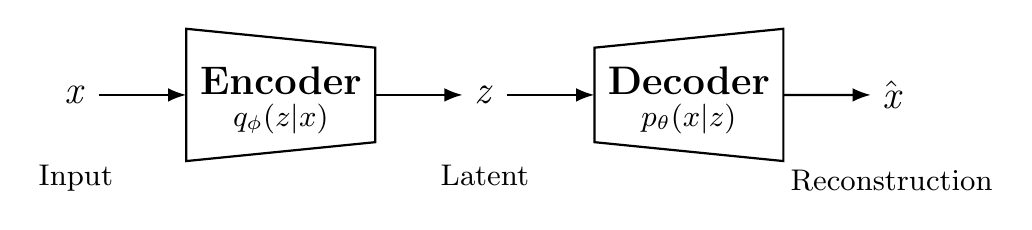
\begin{tikzpicture}[
  node distance=1.8cm,
  >=Latex,
  scale=1.2,
  transform shape,
  every node/.style={font=\large},
  arrow/.style={->, thick}
]

% Variables con texto debajo
\node (x) {\textit{x}};
\node[below=0.4cm of x, font=\small] {Input};

% Encoder (trapecio: ancho a la izquierda, estrecho a la derecha)
\node[right=1.8cm of x] (enc_center) {};
\draw[thick] 
  ([xshift=-1cm, yshift=0.7cm] enc_center.center) -- 
  ([xshift=1cm, yshift=0.5cm] enc_center.center) -- 
  ([xshift=1cm, yshift=-0.5cm] enc_center.center) -- 
  ([xshift=-1cm, yshift=-0.7cm] enc_center.center) -- cycle;
\node[yshift=0.15cm] at (enc_center) {\textbf{Encoder}};
\node[yshift=-0.25cm, font=\small] at (enc_center) {$q_\phi(z|x)$};

% Variable latente
\node[right=1.8cm of enc_center] (z) {\textit{z}};
\node[below=0.4cm of z, font=\small] {Latent};

% Decoder (trapecio: estrecho a la izquierda, ancho a la derecha)
\node[right=1.8cm of z] (dec_center) {};
\draw[thick] 
  ([xshift=-1cm, yshift=0.5cm] dec_center.center) -- 
  ([xshift=1cm, yshift=0.7cm] dec_center.center) -- 
  ([xshift=1cm, yshift=-0.7cm] dec_center.center) -- 
  ([xshift=-1cm, yshift=-0.5cm] dec_center.center) -- cycle;
\node[yshift=0.15cm] at (dec_center) {\textbf{Decoder}};
\node[yshift=-0.25cm, font=\small] at (dec_center) {$p_\theta(x|z)$};

% Reconstrucción
\node[right=1.8cm of dec_center] (xhat) {$\hat{\textit{x}}$};
\node[below=0.4cm of xhat, font=\small] {Reconstruction};

% Flechas
\draw[arrow] (x) -- ([xshift=-1cm] enc_center.center);
\draw[arrow] ([xshift=1cm] enc_center.center) -- (z);
\draw[arrow] (z) -- ([xshift=-1cm] dec_center.center);
\draw[arrow] ([xshift=1cm] dec_center.center) -- (xhat);

\end{tikzpicture}
